\documentclass[letterpaper,12pt]{article}
\usepackage[utf8]{inputenc}
\usepackage{amsmath, amsfonts}
\usepackage[x11names]{xcolor}
\usepackage{pgfplots}
\usepackage{tikz}
\usepackage{braket}

\usetikzlibrary{arrows.meta}
\pgfplotsset{
  compat = newest,
  my_style/.style={
    clip=false,
    view={45}{15},
    width=12cm,height=12cm,
    axis lines=middle,
    axis equal,
    axis line style={Latex-Latex},
    xmin=-1,
    xmax=6,
    ymin=-1,
    ymax=6,
    zmin=-1,
    zmax=6,
    % xlabel={$x$},
    % ylabel={$y$},
    % zlabel={$z$},
    xtick={1, 5},
    ytick={1, 5},
    ztick={1, 5},
    line width=1pt,
  },
}

% remove spacing around date and author
\usepackage{titling}
\predate{}
\postdate{}
\preauthor{}
\postauthor{}

\author{}
\title{MATH 262 - Homework 7.1}
\date{} % clear date

\begin{document}

\maketitle

\begin{enumerate}
  \item[7.]
    Arguing geometrically, find all eigenvectors and eigenvalues of the linear transformation:
    \begin{center}
      Scaling by 5 in $\mathbb{R}^3$
    \end{center}
    Then find an eigenbasis if you can, and thus determine whether the given transformation is diagonalizable. \\
    \\
    Below is a plot of a vector and its scaled counterpart. \\
    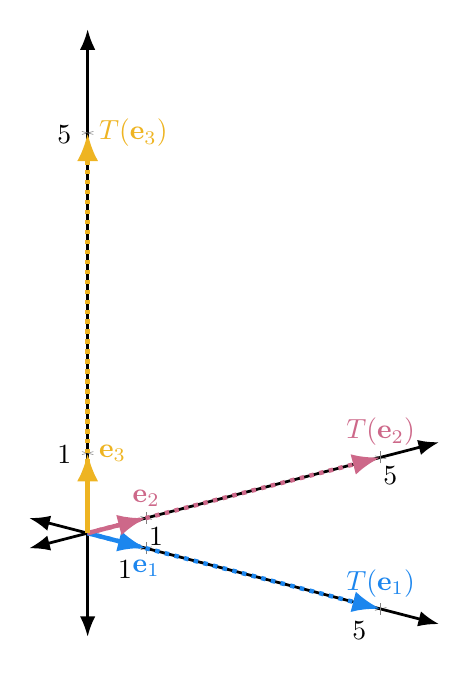
\begin{tikzpicture}
      \begin{axis}[my_style]
        \addplot3[-Latex, DodgerBlue2, ultra thick] coordinates {
          (0, 0, 0)
          (1, 0, 0)
        } node[below,pos=1] {$\mathbf{e}_1$};
        \addplot3[-Latex, DodgerBlue2, ultra thick, dotted] coordinates {
          (0, 0, 0)
          (5, 0, 0)
        } node[above,pos=1] {$T(\mathbf{e}_1)$};

        \addplot3[-Latex, PaleVioletRed3, ultra thick] coordinates {
          (0, 0, 0)
          (0, 1, 0)
        } node[above,pos=1] {$\mathbf{e}_2$};
        \addplot3[-Latex, PaleVioletRed3, ultra thick, dotted] coordinates {
          (0, 0, 0)
          (0, 5, 0)
        } node[above,pos=1] {$T(\mathbf{e}_2)$};

        \addplot3[-Latex, Goldenrod2, ultra thick] coordinates {
          (0, 0, 0)
          (0, 0, 1)
        } node[right,pos=1] {$\mathbf{e}_3$};
        \addplot3[-Latex, Goldenrod2, ultra thick, dotted] coordinates {
          (0, 0, 0)
          (0, 0, 5)
        } node[right,pos=1] {$T(\mathbf{e}_3)$};
      \end{axis}
    \end{tikzpicture} \\
    Notice $T(\mathbf{e}_1) = A\mathbf{e}_1 = 5\mathbf{e}_1$. This follows the form described in the definition of an eigenvalue i.e. a $\lambda$ such that $A\vec{v} = \lambda\vec{v}$. Thus, the eigenvalue is 5. This also holds for $\mathbf{e}_2$ and $\mathbf{e}_3$. Therefore, $\mathbf{e}_1$, $\mathbf{e}_2$, and $\mathbf{e}_3$ form an eigenbasis and all vectors in $\mathbb{R}^3$ are eigenvectors of this transformation.
\end{enumerate}

\end{document}
